
% ******** Meta ******** %

\documentclass{minimal}
\usepackage[ paper=a4paper
           , margin=0.5cm
           ]{geometry}
\usepackage{CJKutf8}

% ******** Envs ******** %

\usepackage{pxrubrica}
\usepackage{tikz}

% ******** Body ******** %

\begin{document}

\begin{CJK}{UTF8}{min}\ruby[m]{課題}{ か| だい}\end{CJK}: \dotfill ~ 
\begin{CJK}{UTF8}{min}\ruby[g]{内容}{ないよう}\end{CJK}: \dotfill ~~~

\hfill

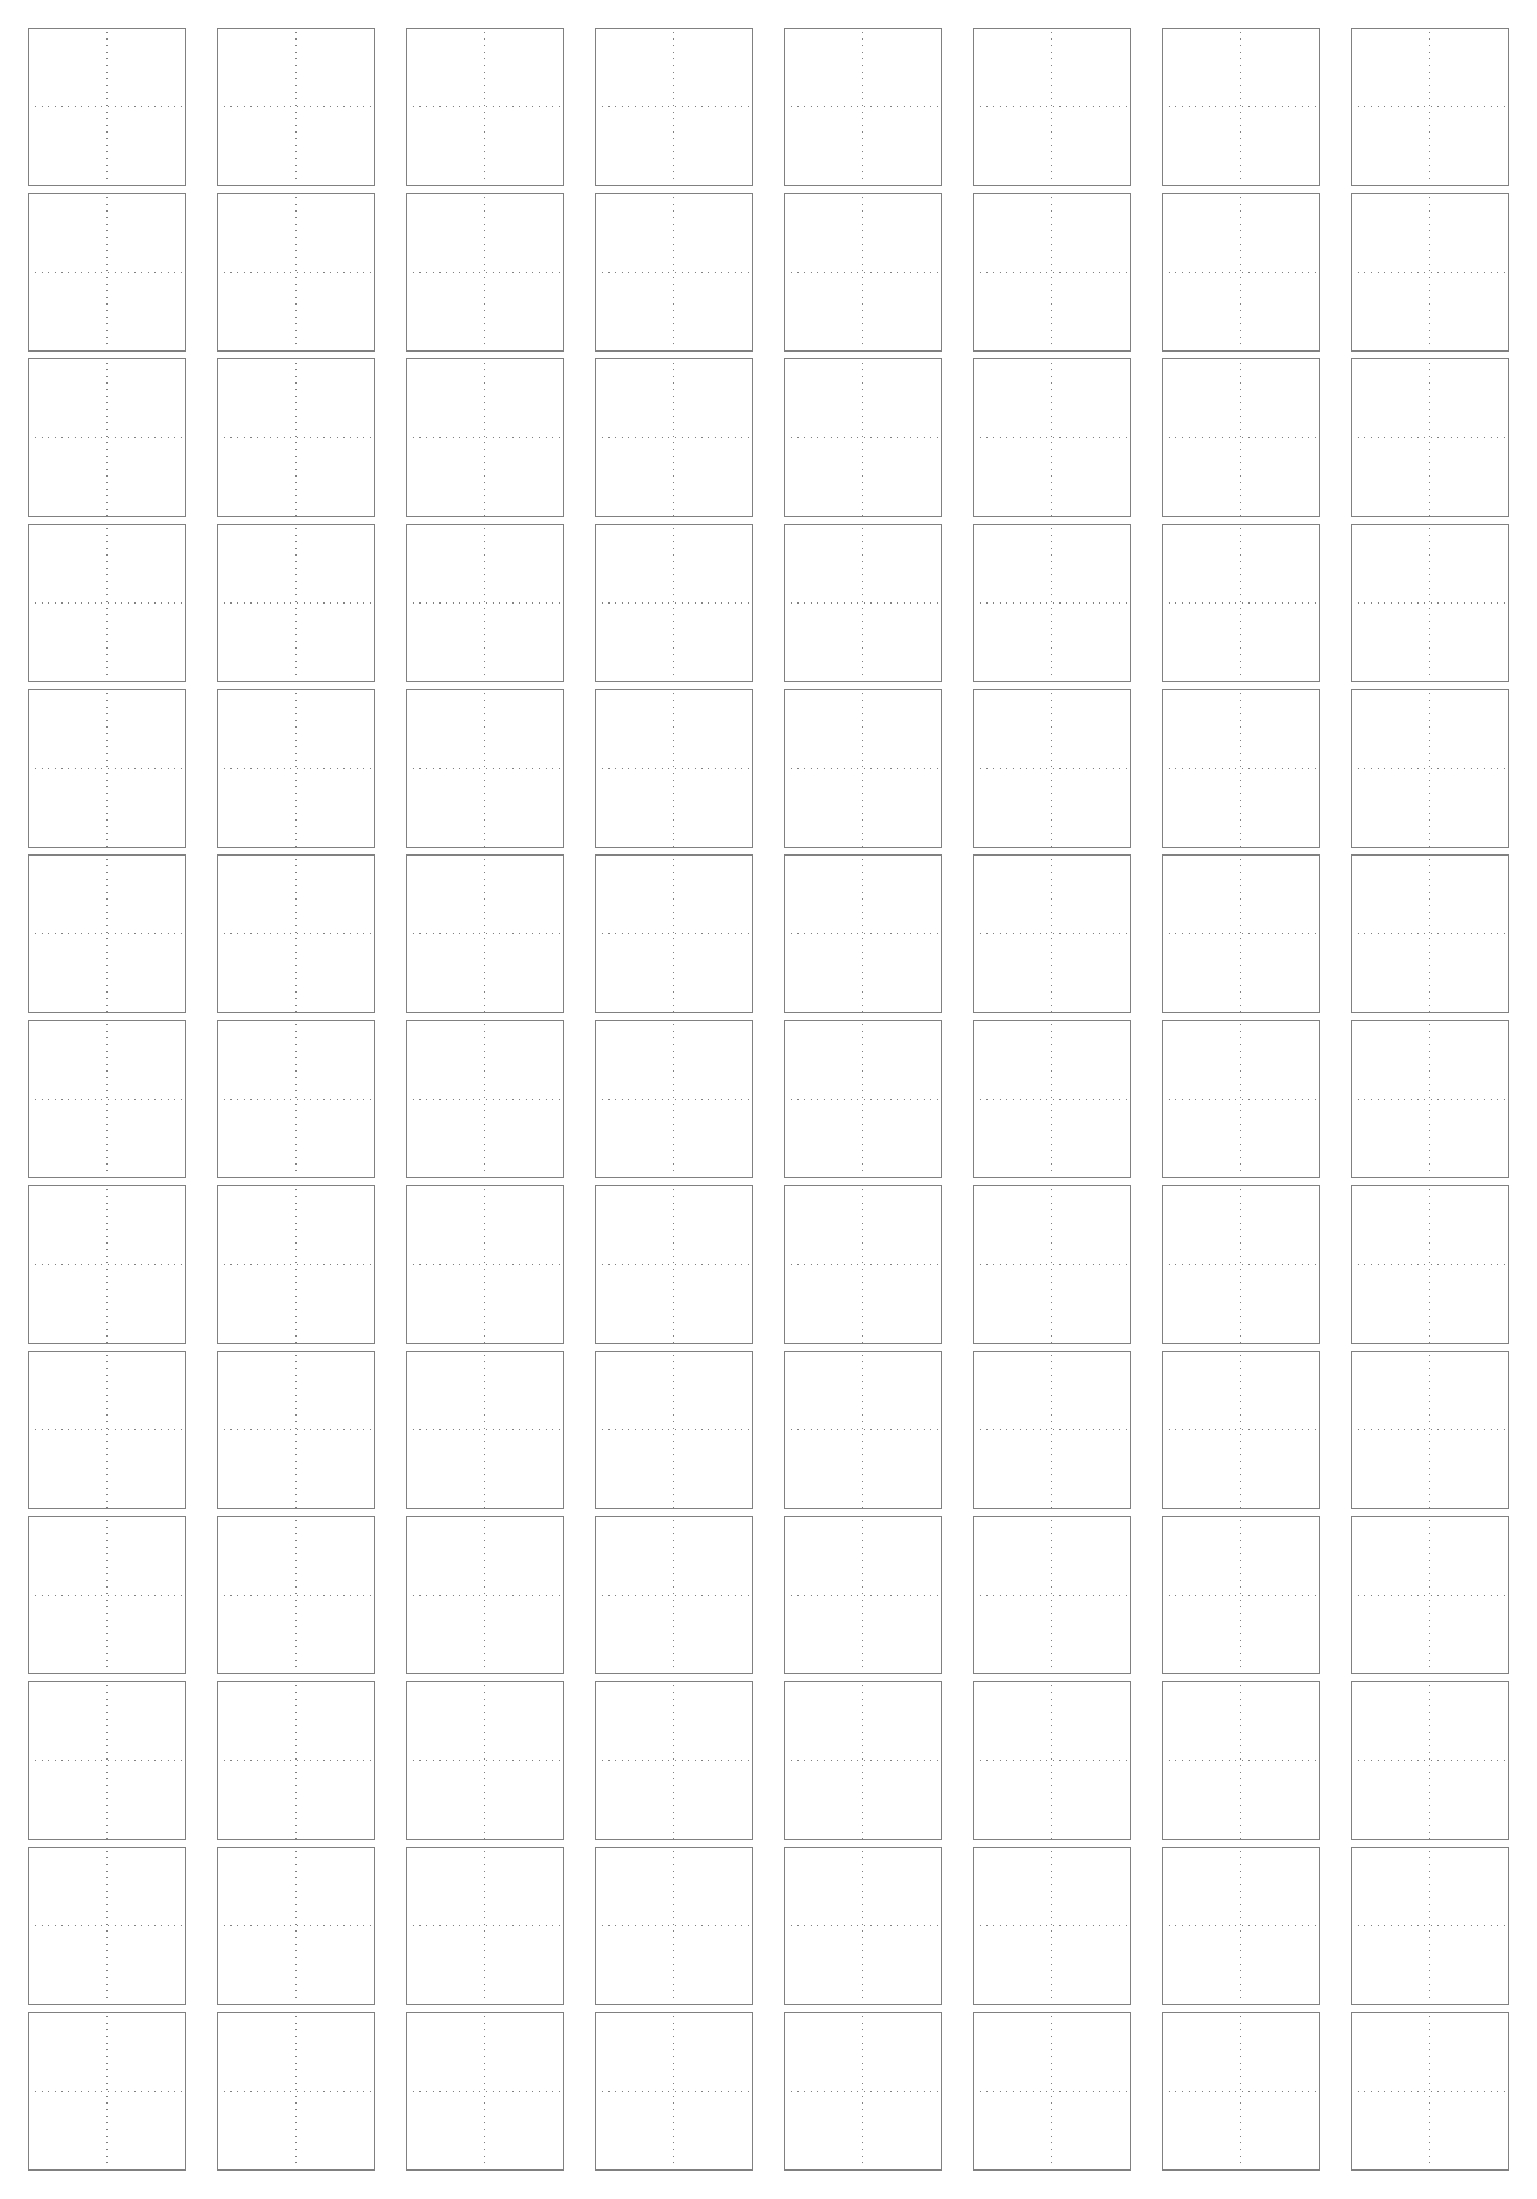
\begin{tikzpicture}
  \foreach \y in {0,2.1,...,26}
    \foreach \x in {0,2.4,...,18} {
      \draw[step=1cm, gray] (\x,\y) rectangle (\x+2,\y+2);
      \draw[dotted, gray] (\x+1,\y) -- (\x+1,\y+2);
      \draw[dotted, gray] (\x,\y+1) -- (\x+2,\y+1);
    }
\end{tikzpicture}

\end{document}  